\chapter{Design}
In this chapter we focus on how to implement what we have specified in the analysis chapter.
First, we describe our application's architecture.
Then, we discuss what technologies were considered for implementing the application, and which of the technologies were chosen and why.
We name our application "Choose well".

\section{Architecture}
\todo[inline]{add footnote}
We design our solution(footnote - from now on we will refer to the whole application as the solution as not to  confuse it with the applications it consists of) as multiple independent single-page applications for better modularity. 
One application is the guest dietary profile editor.
It allows a guest to set their dietary preferences like being allergic to something or being vegetarian.
Another application is the restaurant menu maker.
It serves for restaurant employees to specify their menu's contents.
Last application is the personalized menu viewer for restaurant guests.
It combines information gathered by the other applications to display personalized menus to guests. 
\todo[inline]{add figure number}
\todo[inline]{move bottom border a bit lower}
Figure x contains a depiction of our solution's architecture.

\begin{figure}[h]
  \centering
  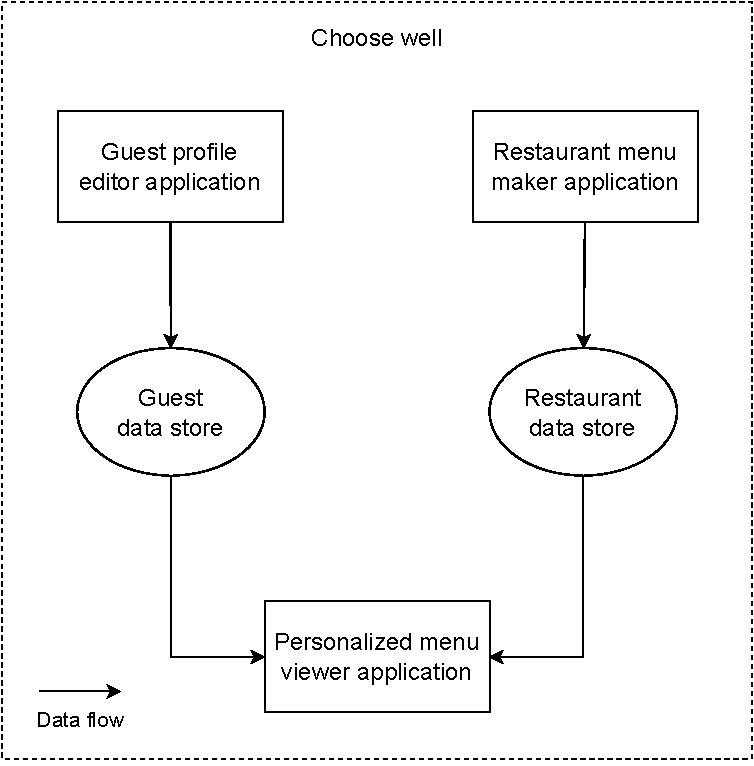
\includegraphics[width=0.62\linewidth]{master-thesis/img/architecture_data_flow.pdf}
  \caption{The solution's architecture}
\end{figure}

\section{Technological stack}
\todo[inline]{add links to technologies - footnotes, link to documentation of the technology}
This section contains an overview of considered tools for implementing the solution.
We also note which ones we chose and why.

\subsection*{User interface}
\todo[inline]{add link}
We chose \textbf{React} for developing the UI of the solution's applications.
This decision was made on the account that Solid is programmed for React.
There even exists a Solid React SDK(link) with a Login button component which can be used for authentication of users.

\subsection*{Programming language}
As for a programming language, JavaScript and TypeScript were considered.
Both languages are supported by React, and we chose \textbf{Typescript} because it adds type control to the programmer's code which makes it less error-prone.

\subsection*{Build tool}
  We need to create the application.
  We need to make the application to a single file that is sent to the client.
  We need to build and deploy our application.

  We considered Vite and Create React App

  Vite (French: [vit], like "veet") is a local development server written by Evan You and used by default by the Vue project templates. It has support for TypeScript and JSX.

  It monitors files as they're being edited and upon file save the web browser reloads the code being edited through a process called Hot Module Replacement (HMR) which works by just reloading the specific file being changed using ES6 modules (ESM) instead of recompiling the entire application.

  Vite is a newer build tool that has gained popularity in recent years. It was created to address the limitations of existing build tools, particularly in the development phase. Vite is a build tool that is optimized for speed. It leverages the latest browser technologies, such as ES modules and native browser imports, to provide fast build times.

  Vite is particularly useful for small to medium-sized projects that do not require complex configurations. It is built on top of the Rollup bundler, which is known for its fast build times. Vite also provides a development server that is optimized for performance. The server leverages HTTP/2 server push, which enables the server to send multiple responses for a single client request.

  Create React App is built on Webpack and Babel and it is a popular tool that enables developers to quickly set up a React project. It is an officially supported tool by the React team, making it a reliable choice. It creates a basic React application with all the necessary configuration files, dependencies, and scripts. The tool provides a pre-configured environment that abstracts away much of the configuration that developers would typically have to handle manually. This means that the developer can focus on writing code rather than configuration files.

  We chose \textbf{Vite} because it is better for deployment process

% end of \subsection

\subsection*{Deployment}
\todo[inline]{add link to GH Pages doc}
  For deployment, only \textbf{GitHub Pages} was considered.

  GitHub Pages is a static site hosting service that takes HTML, CSS, and JavaScript files straight from a repository on GitHub, optionally runs the files through a build process, and publishes a website.

  There are three types of GitHub Pages sites: project, user, and organization. Project sites are connected to a specific project hosted on GitHub, such as a JavaScript library or a recipe collection. User and organization sites are connected to a specific account on GitHub.com.

% end of \subsection

\subsection*{Package manager}
  We need a tool to manage our application's dependencies.
  A package manager can seamlessly handle installing and uninstalling of packages which is another name for JavaScript libraries.

  For package management in our application we consider two options: npm and yarn.

  npm is a package manager for the JavaScript programming language.
  npm is used to fetch any packages that an application needs for development, testing, and/or production, and may also be used to run tests and tools used in the development process.
  It consists of a command line client, also called npm, and an online database of packages, called the npm registry. 
  The registry is accessed via the client, and the available packages can be browsed and searched via the npm website.

  A successful and popular alternative package manager is Yarn. 
  Yarn resolves the dependencies using a different algorithm that can mean a faster user experience.
  More specifically, yarn can download packages in parallel to maximize network utilization.

  Although Yarn is just as good as npm for handling packages, the latter is more widely used.
  For this reason we decide to use \textbf{npm} for our application. 
% end of \subsection

\subsection*{Responsive design}
  Responsive web design or RWD is a web design approach to make web pages render well on all screen sizes and resolutions while ensuring good usability.
  We need our application to be responsive to various device screens.
  We want a mobile-first approach as most people use smartphones these days.
  The chosen tool should be well documented for ease of use.

  Two options were considered, which are Bootstrap, Material UI.
  Let us briefly introduce them.

  Made by myself and Jacob Thornton, Bootstrap is an open-source front-end toolkit created to help designers and developers quickly and efficiently build awesome stuff online. Our goal is to provide a refined, well-documented, and extensive library of flexible design components built with HTML, CSS, and JavaScript for others to build and innovate on.

  The most prominent components of Bootstrap are its layout components, as they affect an entire web page. The basic layout component is called "Container", as every other element in the page is placed in it.

  Once a container is in place, other Bootstrap layout components implement a CSS Flexbox layout through defining rows and columns.

  Material Design is a design language which uses grid-based layouts, responsive animations and transitions, padding, and depth effects such as lighting and shadows.

  The main purpose of Material Design is the creation of a visual language that combines principles of good design with technical and scientific innovation. 

  Designers optimize users' experience with 3D effects, realistic lighting and animation features in immersive, platform-consistent GUIs.

  We decide to opt for \textbf{Bootstrap} as it is easier to use and well documented.
% end of \subsection

\subsection*{Persistence}
Our application needs to store and later read data.
We decide to use the \textbf{Solid} technology for this purpose. 

\subsection*{Documentation}
\todo[inline]{add links to docs in footnote}
We need to capture how our application works for users and future developers.
Programmer documentation is available as several simple HTML pages created using \textbf{GitHub markdown}.
User documentation is in a form of a webpage which is hosted on \textbf{GitHub Pages}.

\subsection*{Authentication}
For authentication purposes, the Inrupt's solid-client JavaScript library is used.
We also use the Inrupt's React SDK which contains a Login component which uses the aforementioned library implicitly.

\todo[inline]{add testing}
% \subsection*{Testing}
% We need to test our application in order to prevent bugs during implementation.
% % https://legacy.reactjs.org/docs/testing-environments.html
